%
\section{Experimental Results}
\label{sec:results}
%

\begin{table}[tb]
  \caption{Submariner Results}
  \label{tab:submariner_results}
  \resizebox{\linewidth}{!}{%
    \begin{tabular}{@{}llccc@{}}
      \toprule
      \textbf{Database} & \textbf{Forwarding Tool} & \textbf{Response Time (ms)} & \textbf{Availability (\%)} & \textbf{Resource Usage (MB)} \\
      \midrule
      \multirow{2}{*}{Postgres (Operator)} 
          & Submariner     & XX.XX & XX.XX & XX \\
          & Clustershift   & XX.XX & XX.XX & XX \\
      \midrule
      \multirow{2}{*}{Postgres (Vanilla)} 
          & Submariner     & XX.XX & XX.XX & XX \\
          & Clustershift   & XX.XX & XX.XX & XX \\
      \midrule
      \multirow{2}{*}{MongoDB (Operator)} 
          & Submariner     & XX.XX & XX.XX & XX \\
          & Clustershift   & XX.XX & XX.XX & XX \\
      \midrule
      \multirow{2}{*}{MongoDB (Vanilla)} 
          & Submariner     & XX.XX & XX.XX & XX \\
          & Clustershift   & XX.XX & XX.XX & XX \\
      \bottomrule
    \end{tabular}
  }
\end{table}

\begin{table}[tb]
  \caption{Results of Forwarding and Connectivity Tool Combinations}
  \label{tab:forwarding_connectivity_results}
  \resizebox{\linewidth}{!}{%
    \begin{tabular}{@{}lll l ccc@{}}
      \toprule
      \textbf{Connectivity Tool} & \textbf{Database} & \textbf{Deployment} & \textbf{Forwarding Tool} 
        & \textbf{Response Time (ms)} & \textbf{Availability (\%)} & \textbf{Resource Usage (MB)} \\
      \midrule

      \multirow{8}{*}{Submariner} 
        & \multirow{4}{*}{Postgres} 
          & Operator    & Clustershift & -- & -- & -- \\
        &                                   & Operator    & Submariner   & -- & -- & -- \\
        &                                   & StatefulSet & Clustershift & -- & -- & -- \\
        &                                   & StatefulSet & Submariner   & -- & -- & -- \\
        \cmidrule(lr){2-7}
        & \multirow{4}{*}{MongoDB} 
          & Operator    & Clustershift & -- & -- & -- \\
        &                                   & Operator    & Submariner   & -- & -- & -- \\
        &                                   & StatefulSet & Clustershift & -- & -- & -- \\
        &                                   & StatefulSet & Submariner   & -- & -- & -- \\
      \midrule

      \multirow{8}{*}{Skupper} 
        & \multirow{4}{*}{Postgres} 
          & Operator    & Clustershift & -- & -- & -- \\
        &                                   & Operator    & Skupper      & -- & -- & -- \\
        &                                   & StatefulSet & Clustershift & -- & -- & -- \\
        &                                   & StatefulSet & Skupper      & -- & -- & -- \\
        \cmidrule(lr){2-7}
        & \multirow{4}{*}{MongoDB} 
          & Operator    & Clustershift & -- & -- & -- \\
        &                                   & Operator    & Skupper      & -- & -- & -- \\
        &                                   & StatefulSet & Clustershift & -- & -- & -- \\
        &                                   & StatefulSet & Skupper      & -- & -- & -- \\
      \bottomrule
    \end{tabular}
  }
\end{table}

% CPU and Memory Utilization
% TODO: Zu genau? soll etwas weggelassen werden?
% TODO: Nochmal die utilization des target cluster messen und in die Grafik einbauen
\begin{figure}[t]
    \centering
    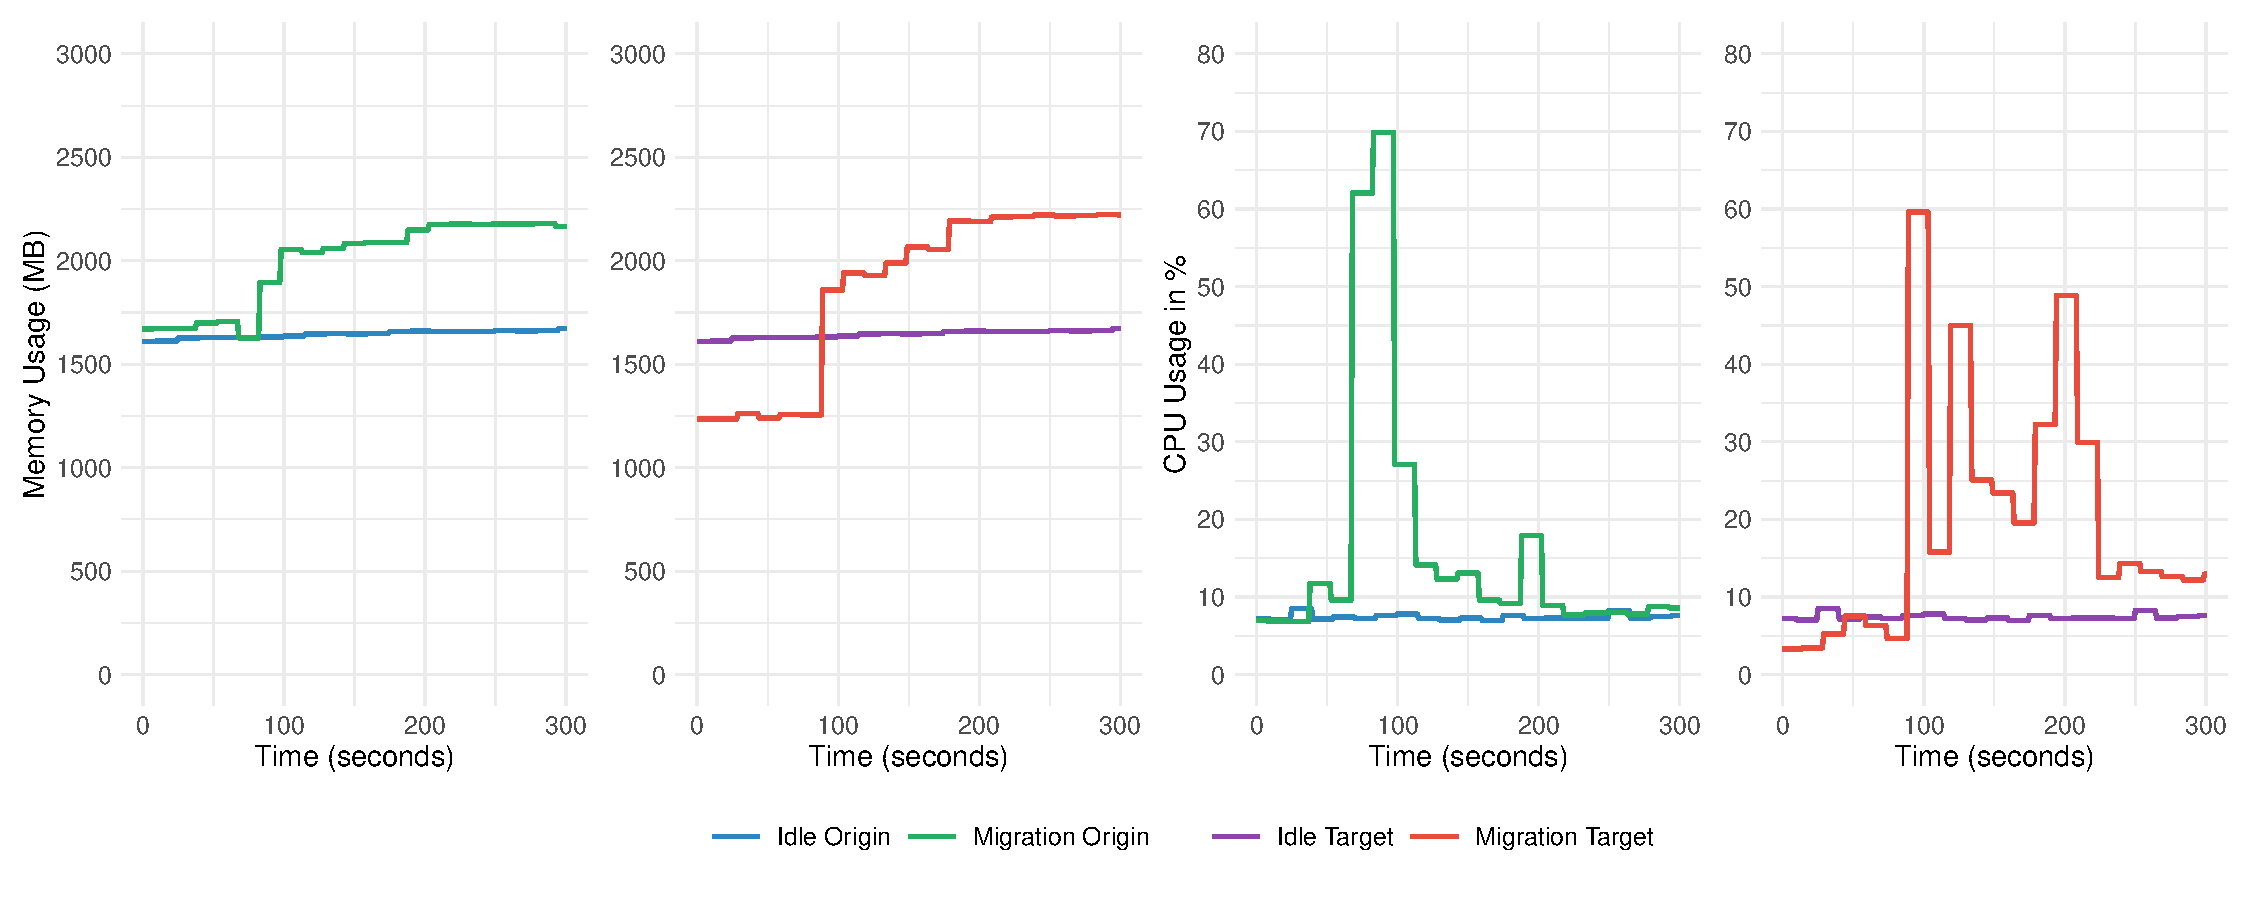
\includegraphics[width=\linewidth]{figures/util-metrics.pdf}
    \caption{CPU and Memory Utilization of \textit{Clusters}. 
    }
    \label{fig:cpu-and-memory-utilization}
\end{figure}
% 
Figure~\ref{fig:cpu-and-memory-utilization} shows the CPU and memory utilization of the origin and target clusters during the idle and migration states.
Idle corresponds to normal cluster load with no migration components, while migration includes the deployment of the migration components and the execution of the migration process. 
In the origin cluster, at about $30$ seconds, a small spike in memory usage can be observed.
This reflects the deployment of the Submariner Broker and Operator, which requires about $30$\,MB additional memory. 
A similar increase can be observed in the target cluster at roughly $40$ seconds.
The CPU utilization also experiences an increase due to the deployment of the Submariner resources.
It increases from approximately $6.85\%$ to a peak of $11.75\%$ on the source cluster and from $3.45\%$ to a peak of $7.55\%$ on the target cluster.
At 100 seconds the most significant jump in both CPU and memory utilization is noticed. 
This corresponds to the replication of the PostgreSQL database.
A memory spike of $430$\,MB on the source cluster and $XXX$\,MB on the target cluster is observed.
Both clusters experience a peak memory load of approximately $2200$\,MB, which remains until the end of the experiment.
On the CPU side, the origin cluster peaks at $70\%$ utilization, while the target cluster peaks at $60\%$.
Both peaks are also caused by the replication of the database.
After the completion of the migration process the replica database is promoted to primary and the original primary is demoted and decoupled from the target database.
This results in a drop in the CPU utilization to about $8\%$ on the origin cluster and $13\%$ on the target cluster, which stays this way.

% Response time
% TODO: muss auf die outliers eingegangen werden?
\begin{figure}[t]
    \centering
    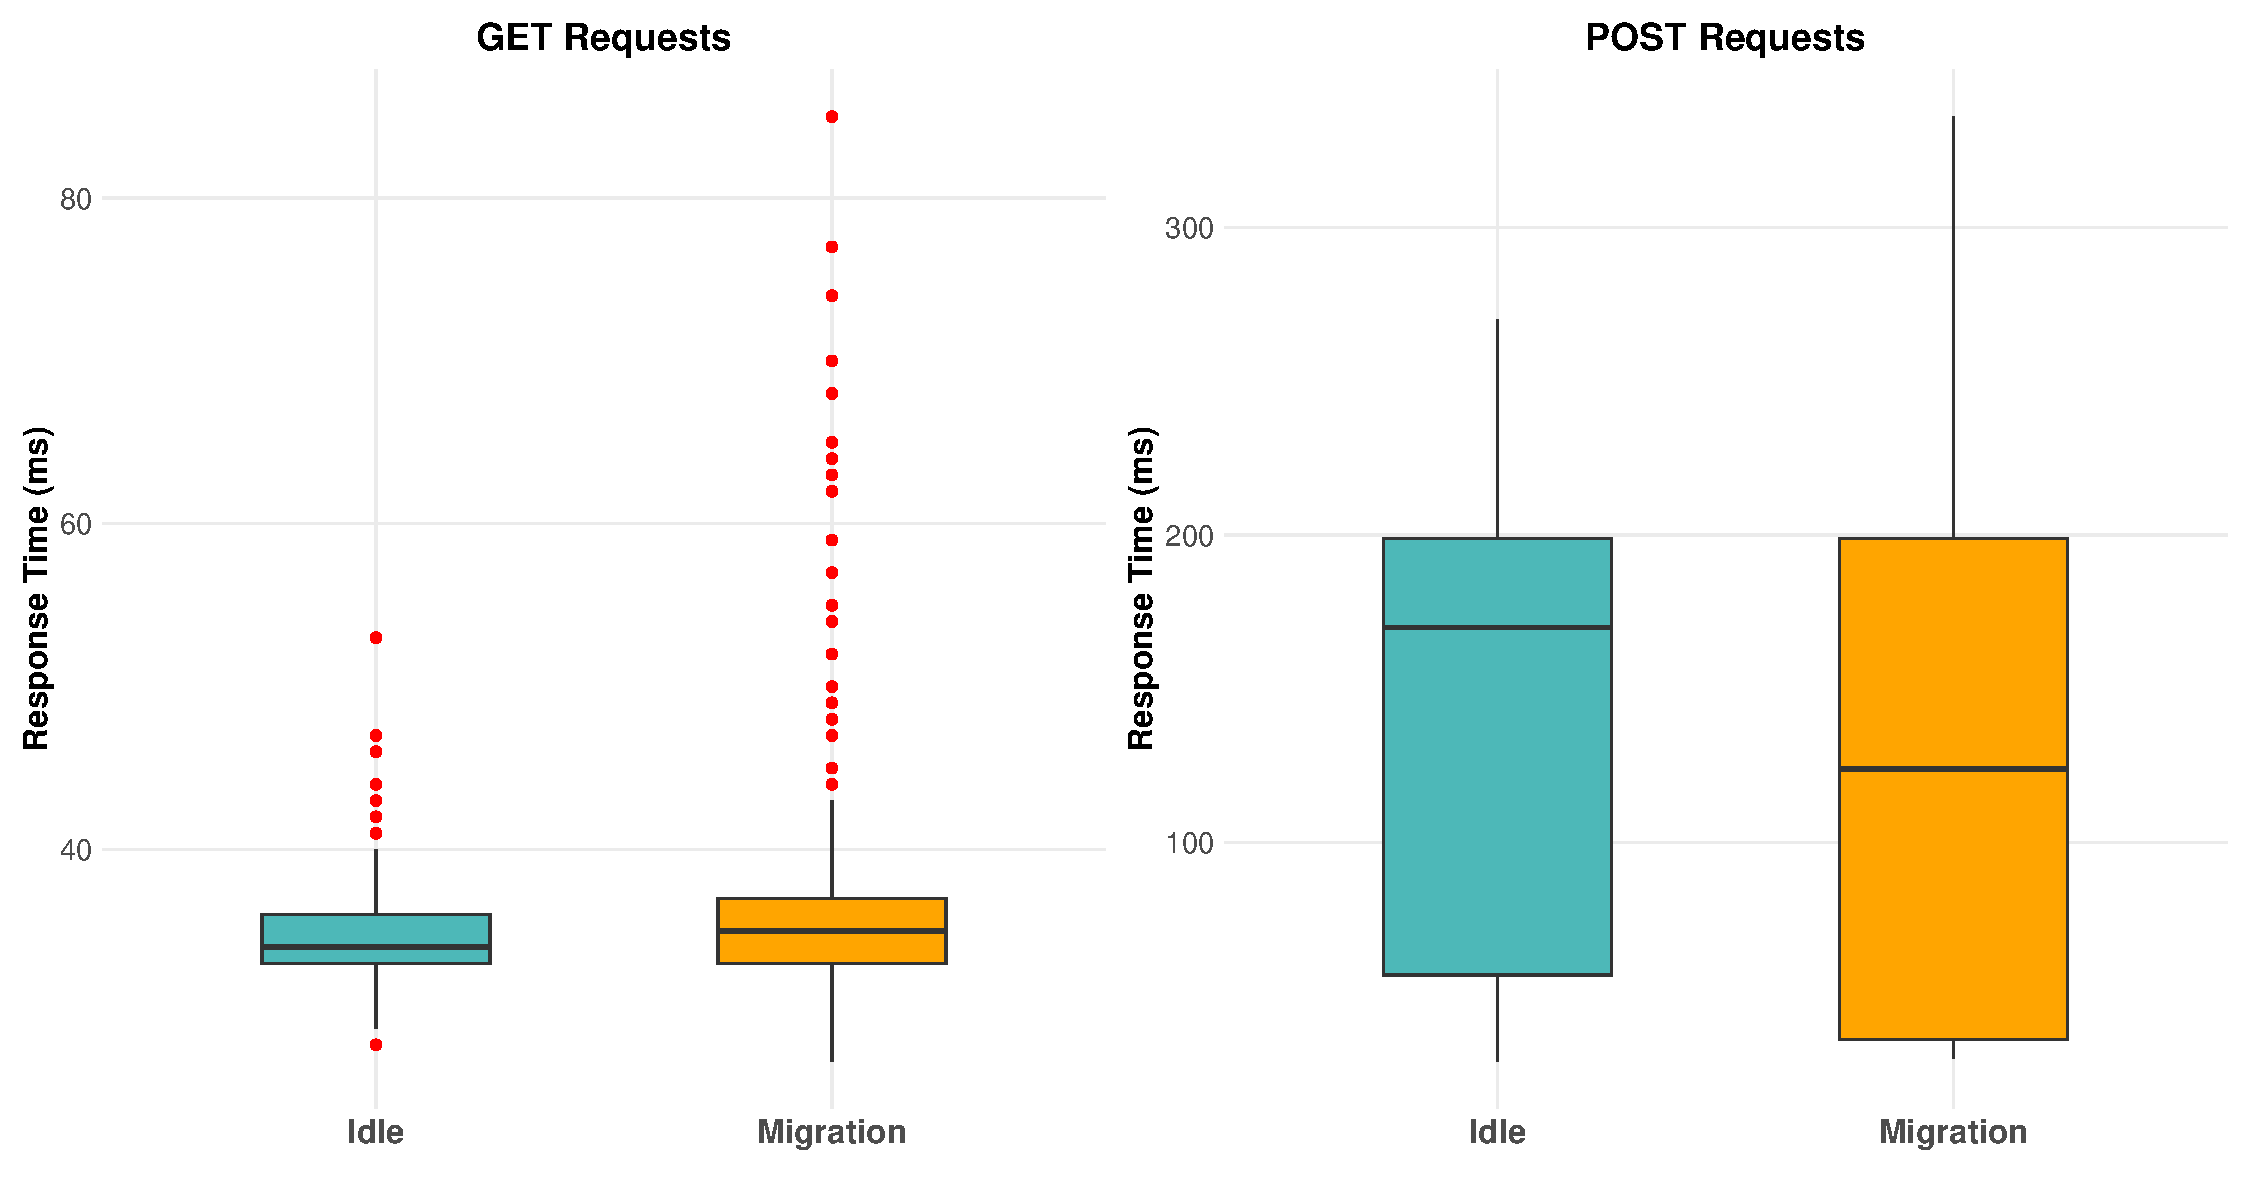
\includegraphics[scale=0.3]{figures/response-time.pdf}
    \caption{Response time of \textit{Clusters}. 
    }
    \label{fig:response-time}
\end{figure}
%
Figure~\ref{fig:response-time} shows the response time of our deployed test application comparing idle and migration states for GET and POST requests.
In the idle state the average response time for GET requests is $34.5$ ms ($\sigma=2.83$).
While migration the average response time for a GET requests increases to $35.9$ ms ($\sigma=6.16$).
For POST requests, the average response time during idle is $133.47$ms ($\sigma=69.76$), while during migration, it decreases slightly to $118.17$ms ($\sigma=74.23$).

% Availability and Downtime
% TODO: Quelle für die ratio?
To evaluate availability and downtime during the migration we check the number of failed requests and their timestamps.
A total of $2165$ requests were sent, with approximately $70\%$ being POST requests and $30\%$ being GET requests.
This is equivalent to $650$ GET requests and $1515$ POST requests.
Out of $650$ GET requests, $12$ failed ($1.85\%$). 
A request counted as failed if the client receiving an HTTP status code outside the $200$ range. 
For POST requests, $29$ out of $1515$ failed ($1.91\%$).
The amount of failed post requests were determined by looking if the database contained the unique message sent by the client. 
Overall $41$ out of the $2165$ sent requests failed, resulting in an availability of $98,11\%$. 
The total downtime during the migration was $4.66$ seconds. 
This was calculated by looking at the timestamps of failed requests.
